\input{./_path-to-root.ltx}
\documentclass[\PathToRoot/\ProjectName]{subfiles}
\whenstandalone{\externaldocument{\PathToRoot/\ProjectName}}

\begin{document}

\begin{figure}[H]
  \centering
  \caption{Model performance with and without splurge factor}
  \whenintegrated{\label{fig:splurge0_Norwayestimation}} 
  \noindent\begin{minipage}{\textwidth}
    \centering
    \begin{subfigure}[b]{.5\linewidth}
      \centering
      % Original path: \PathToRoot/Code/HA-Models/Target_AggMPCX_LiquWealth/Figures/AggMPC_LotteryWin_comparison_splurge0
      \includegraphics[width=\linewidth,height=!,keepaspectratio]{\PathToRoot/images/AggMPC_LotteryWin_comparison_splurge0}
      \caption{Spending dynamics comparison}
      \whenintegrated{\label{fig:aggmpclotterywin_splurge0}} 
    \end{subfigure}
    %
    \begin{subfigure}[b]{.5\linewidth}
      \centering
      % Original path: \PathToRoot/Code/HA-Models/Target_AggMPCX_LiquWealth/Figures/LiquWealth_Distribution_comparison_splurge0
      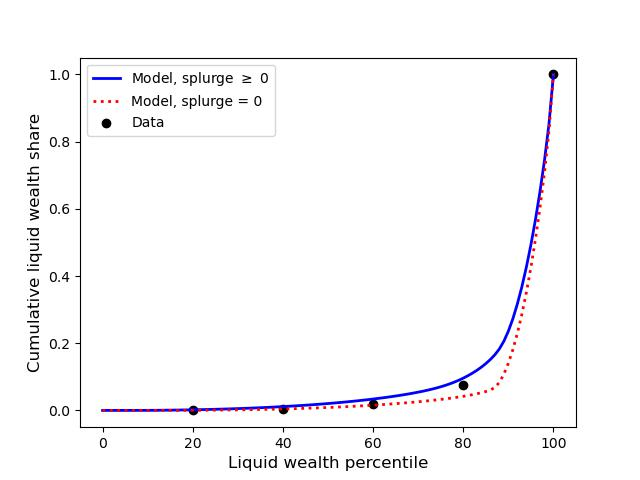
\includegraphics[width=\linewidth,height=!,keepaspectratio]{\PathToRoot/images/LiquWealth_Distribution_comparison_splurge0}
      \caption{Wealth distribution comparison}
      \whenintegrated{\label{fig:liquwealthdistribution_splurge0}} 
    \end{subfigure}
  \end{minipage}
\end{figure}
\noindent\parbox{\textwidth}{
  \medskip
  \footnotesize \textbf{Note}: This figure compares model performance with and without the splurge factor (Appendix~\ref{app:Model-without-splurge}).
  Subfigure~(a) shows the fit to dynamic consumption response from \cite{fagereng-mpc-2021};
  the model without splurge achieves high initial MPC through wider discount factor distribution
  ($\beta = 0.921, \nabla = 0.116$) versus the baseline model ($\beta = 0.968, \nabla = 0.0578$).
  However, it exhibits higher spending propensity in year 2 due to faster spending by borrowing-constrained agents.
  Subfigure~(b) shows the liquid wealth distribution fit; the no-splurge model generates
  more unequal wealth distribution relative to baseline and empirical data from the 2004 SCF.
  While both models perform reasonably well, the splurge factor provides superior empirical fit.
}
\medskip\medskip

% Bibliography inclusion handled automatically by document structure
% The \smartbib command has built-in guards to prevent duplication when included in other documents
\smartbib

\end{document}
